\chapter{Performance Evaluation}\label{sec:evaluation}

In this chapter, we evaluate the performances of non-private GBDT and differentially private GBDT. For the latter, we compare our 2-nodes algorithm versus the classic depth-first tree induction algorithm. We use 3 real datasets not related to cyber insurance, and 4 synthetic cyber insurance datasets (since no real publicly released datasets are available). For the real datasets, we follow the literature and report the root mean square error (RMSE) for regression tasks, and the test error (in \%) for classification tasks. For the synthetic datasets, we report the mean absolute percentage error (MAPE, in \%).

\section{Datasets}

We evaluate the different models on the following datasets:

\begin{itemize}
	\item Abalone\footnote{\href{https://archive.ics.uci.edu/ml/datasets/abalone}{https://archive.ics.uci.edu/ml/datasets/abalone}}: each instance describes attributes of an abalone, such as their sex, length, or weight. The prediction task is a regression task, consisting in predicting the age of the abalone. There are 8 features and 4177 instances.
	\item YearPredictionMSD\footnote{\href{https://archive.ics.uci.edu/ml/datasets/YearPredictionMSD}{https://archive.ics.uci.edu/ml/datasets/YearPredictionMSD}}: each instance describes audio features. The prediction task in a regression task, consisting in predicting the year of release of the song. There are 90 features and 515345 instances. 
	\item Adult\footnote{\href{https://archive.ics.uci.edu/ml/datasets/adult}{https://archive.ics.uci.edu/ml/datasets/adult}}: each instance gives information about the background and education of a person. The prediction task is a classification task, consisting in predicting whether a person makes more than $50k\$$ a year or not. There are 14 features and 48842 instances.
	\item Synthetic\_\{A, B, C, D\}: synthetic datasets generated according to Algorithm ~\ref{algo:generate_data}. Each dataset contains 1 million samples, and there are 28 features per instance. The prediction task is a regression task (refer to Chapter ~\ref{chap:synthetic_data} for more details).
\end{itemize}

For each dataset, we take a sample of $n = 5000$ instances. For the real datasets, we fix the tree depth to $d_{max} = 6$, the learning rate to $\eta = 0.1$ and the number of trees to $n_{trees} = 50$. For the synthetic datasets, we fix $d_{max} = 15, \; \eta = 0.5$ and $n_{trees} = 20$. The models are evaluated through a 5-cross validation process. We report results for the vanilla GBDT (non-private, as in Algorithm ~\ref{algo:gbdt}) and the differentially private GBDT algorithms (depth-first and 2-nodes variants, as in Algorithm ~\ref{algo:dp_gbdt} and ~\ref{algo:2_nodes_dpgbdt} respectively).

\newpage

\section{Results}

We use values of $\epsilon$ in the $[0.1, \ 1.[$ range. Intuitively, the higher the privacy budget $\epsilon$ is, the less noise will be added to the model. This results in better accuracy, but in lower privacy guarantees. We choose not to evaluate the model on higher privacy budgets, as the existing literature (e.g. \cite{dpgbdt}) reports great accuracy in such settings already. 

Table ~\ref{table:training_time} shows the mean training time (in seconds) per tree and per dataset. The depth-first variant implements the algorithm outlined in \cite{dpgbdt}, while the 2-nodes variant tries to enhance it. For the Abalone and YearPredictionMSD datasets, we report the root mean square error (RMSE) for our model. For the Adult dataset, we report the test error (in \%). 

\begin{center}\begin{table}[h!]
	\center
	\noindent\makebox[0pt]{}{
		\begin{tabular}{|c|c|c|c|}
 		\hline
 		 & (Non-DP) Vanilla & (DP) Depth-first & (DP) 2-nodes \\ [0.5ex] \hline\hline
 		Abalone & 2.44 & 0.26 & 0.33 \\ \hline
 		YearPredictionMSD & 85.3 & 11.92 & 12.06 \\ \hline
 		Adult & 0.87 & 0.17 & 0.16 \\ \hline
 		Synthetic A & 0.37 & 0.40 & 0.42 \\ \hline
 		Synthetic B & 0.30 & 0.41 & 0.41 \\ \hline
 		Synthetic C & 0.68 & 0.41 & 0.41 \\ \hline
 		Synthetic D & 0.27 & 0.40 & 0.40 \\ \hline
	\end{tabular}
	\caption{\label{table:training_time} Mean training time (in seconds) per decision tree, for all datasets.}}
\end{table}\end{center}

\begin{figure}[h!]
  \begin{subfigure}{\linewidth}
  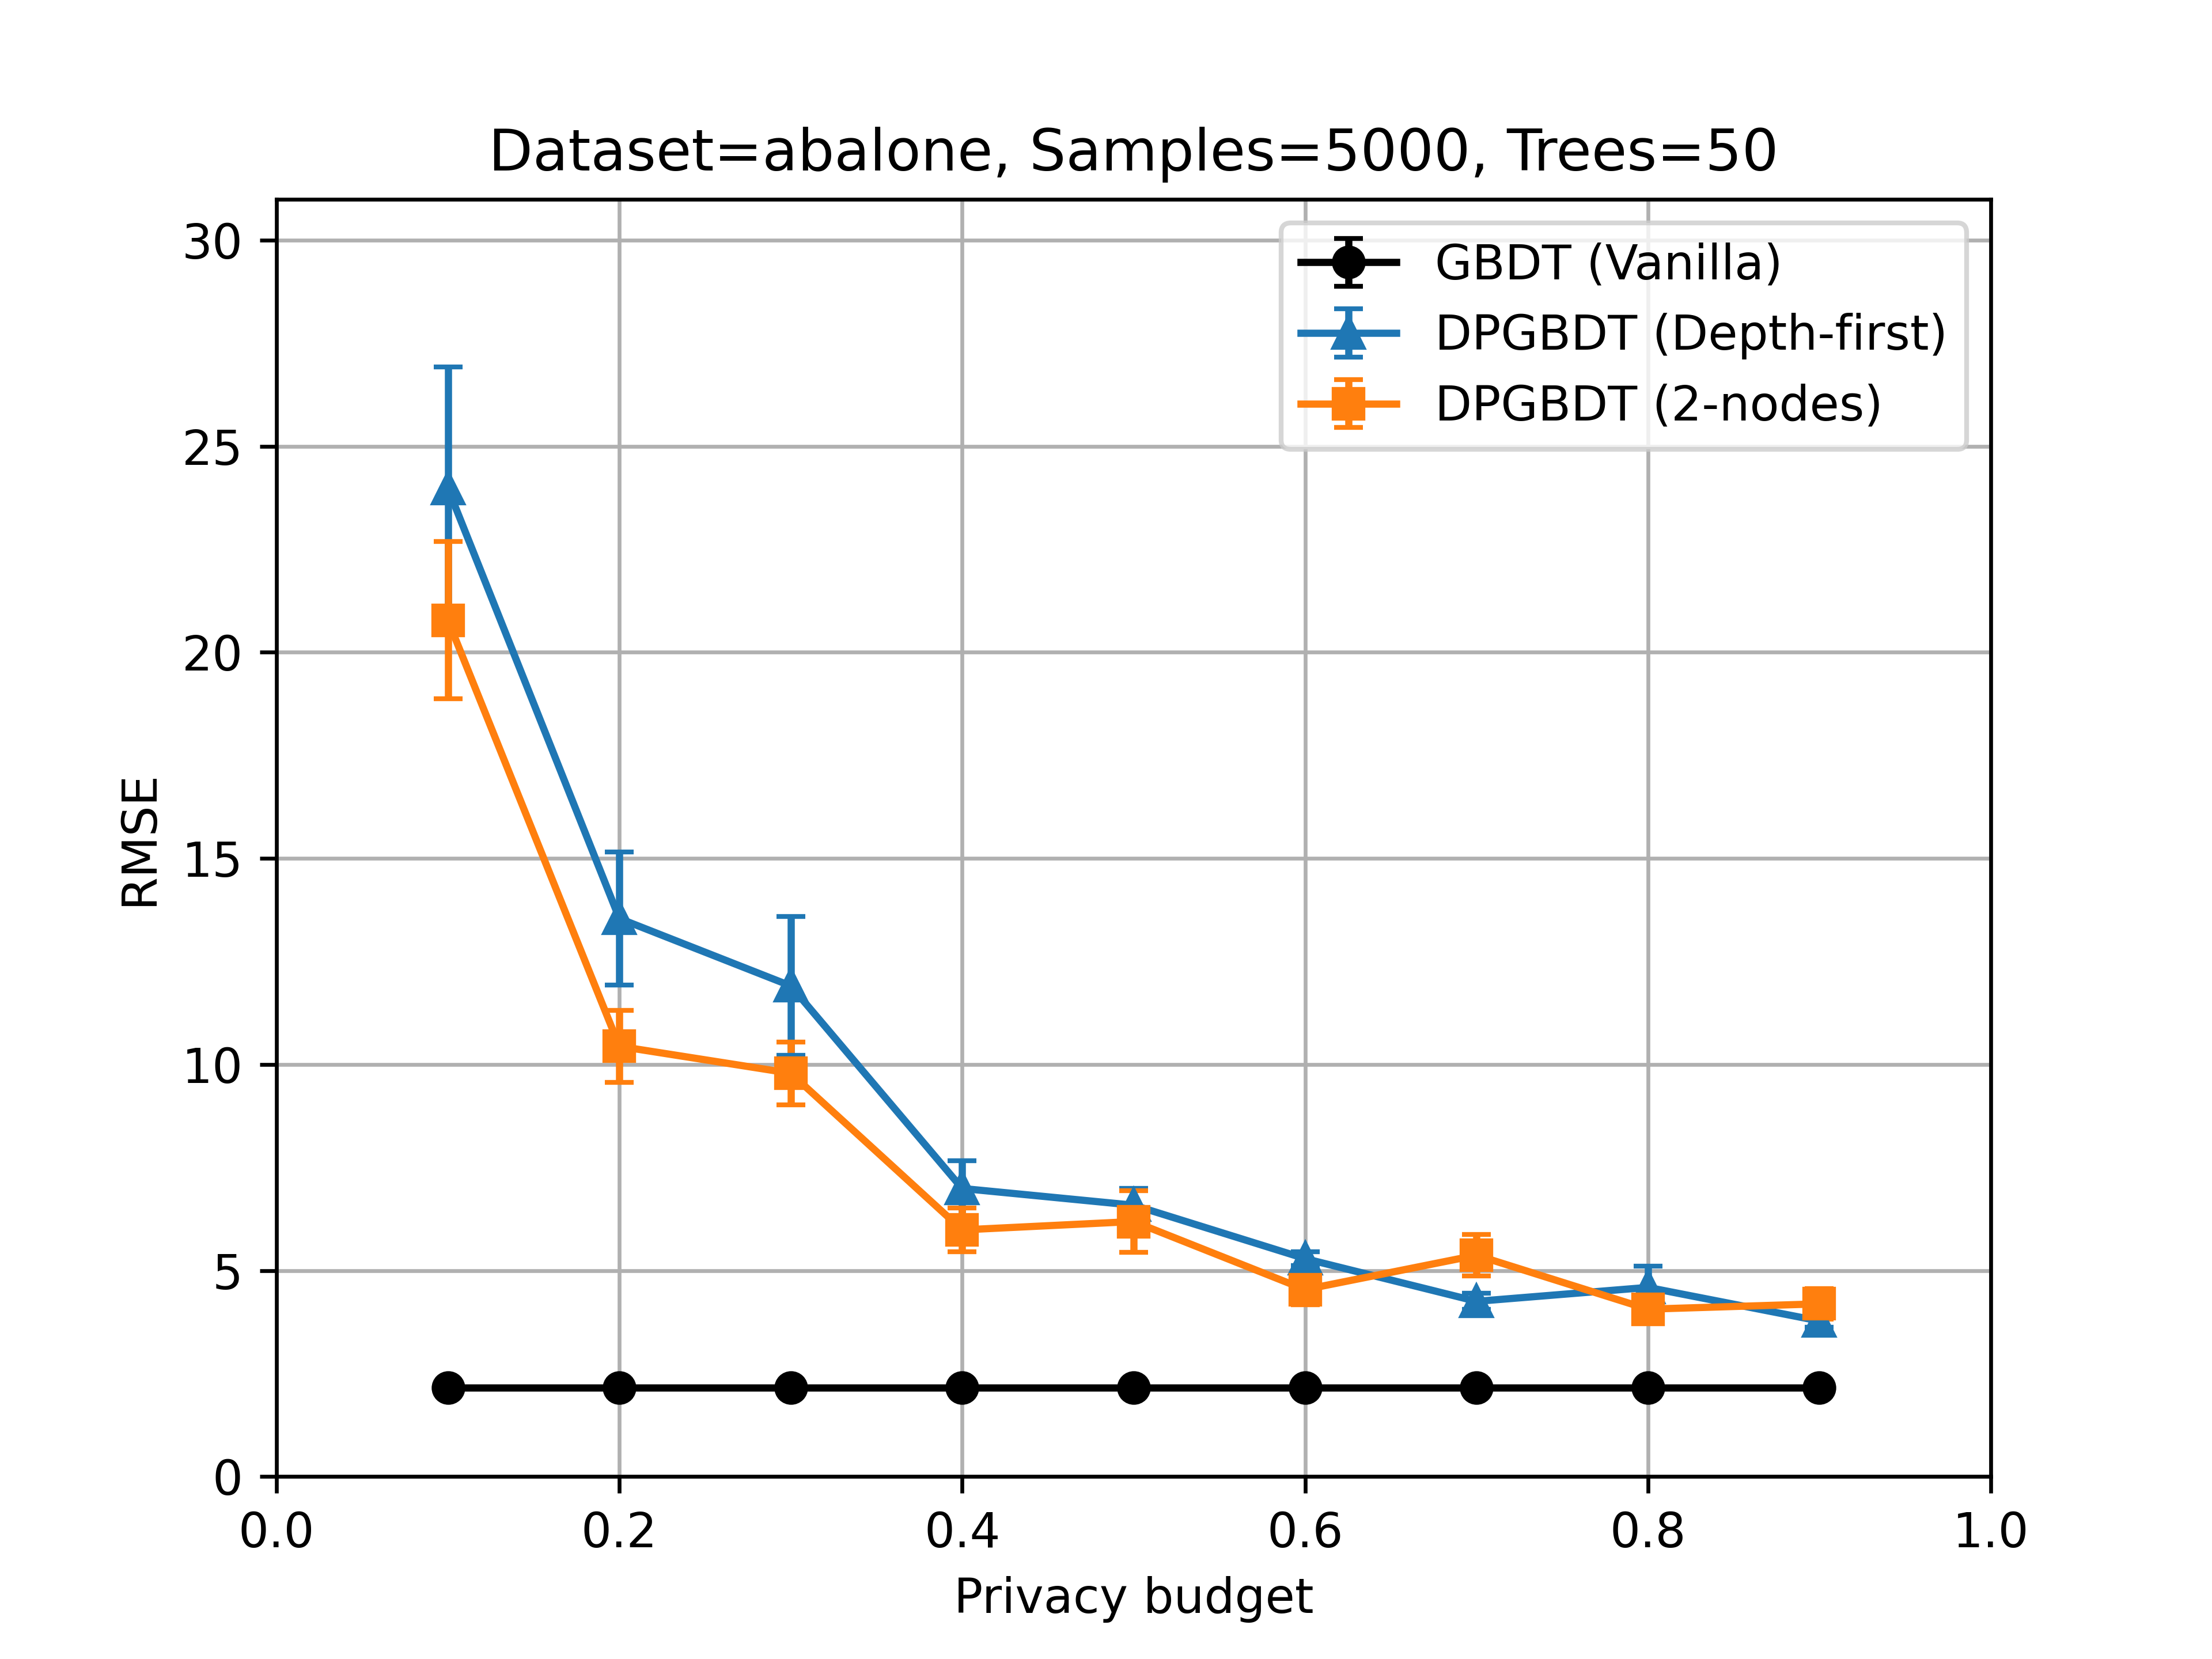
\includegraphics[width=.5\linewidth]{images/evaluation/abalone_5000.png}\hfill
  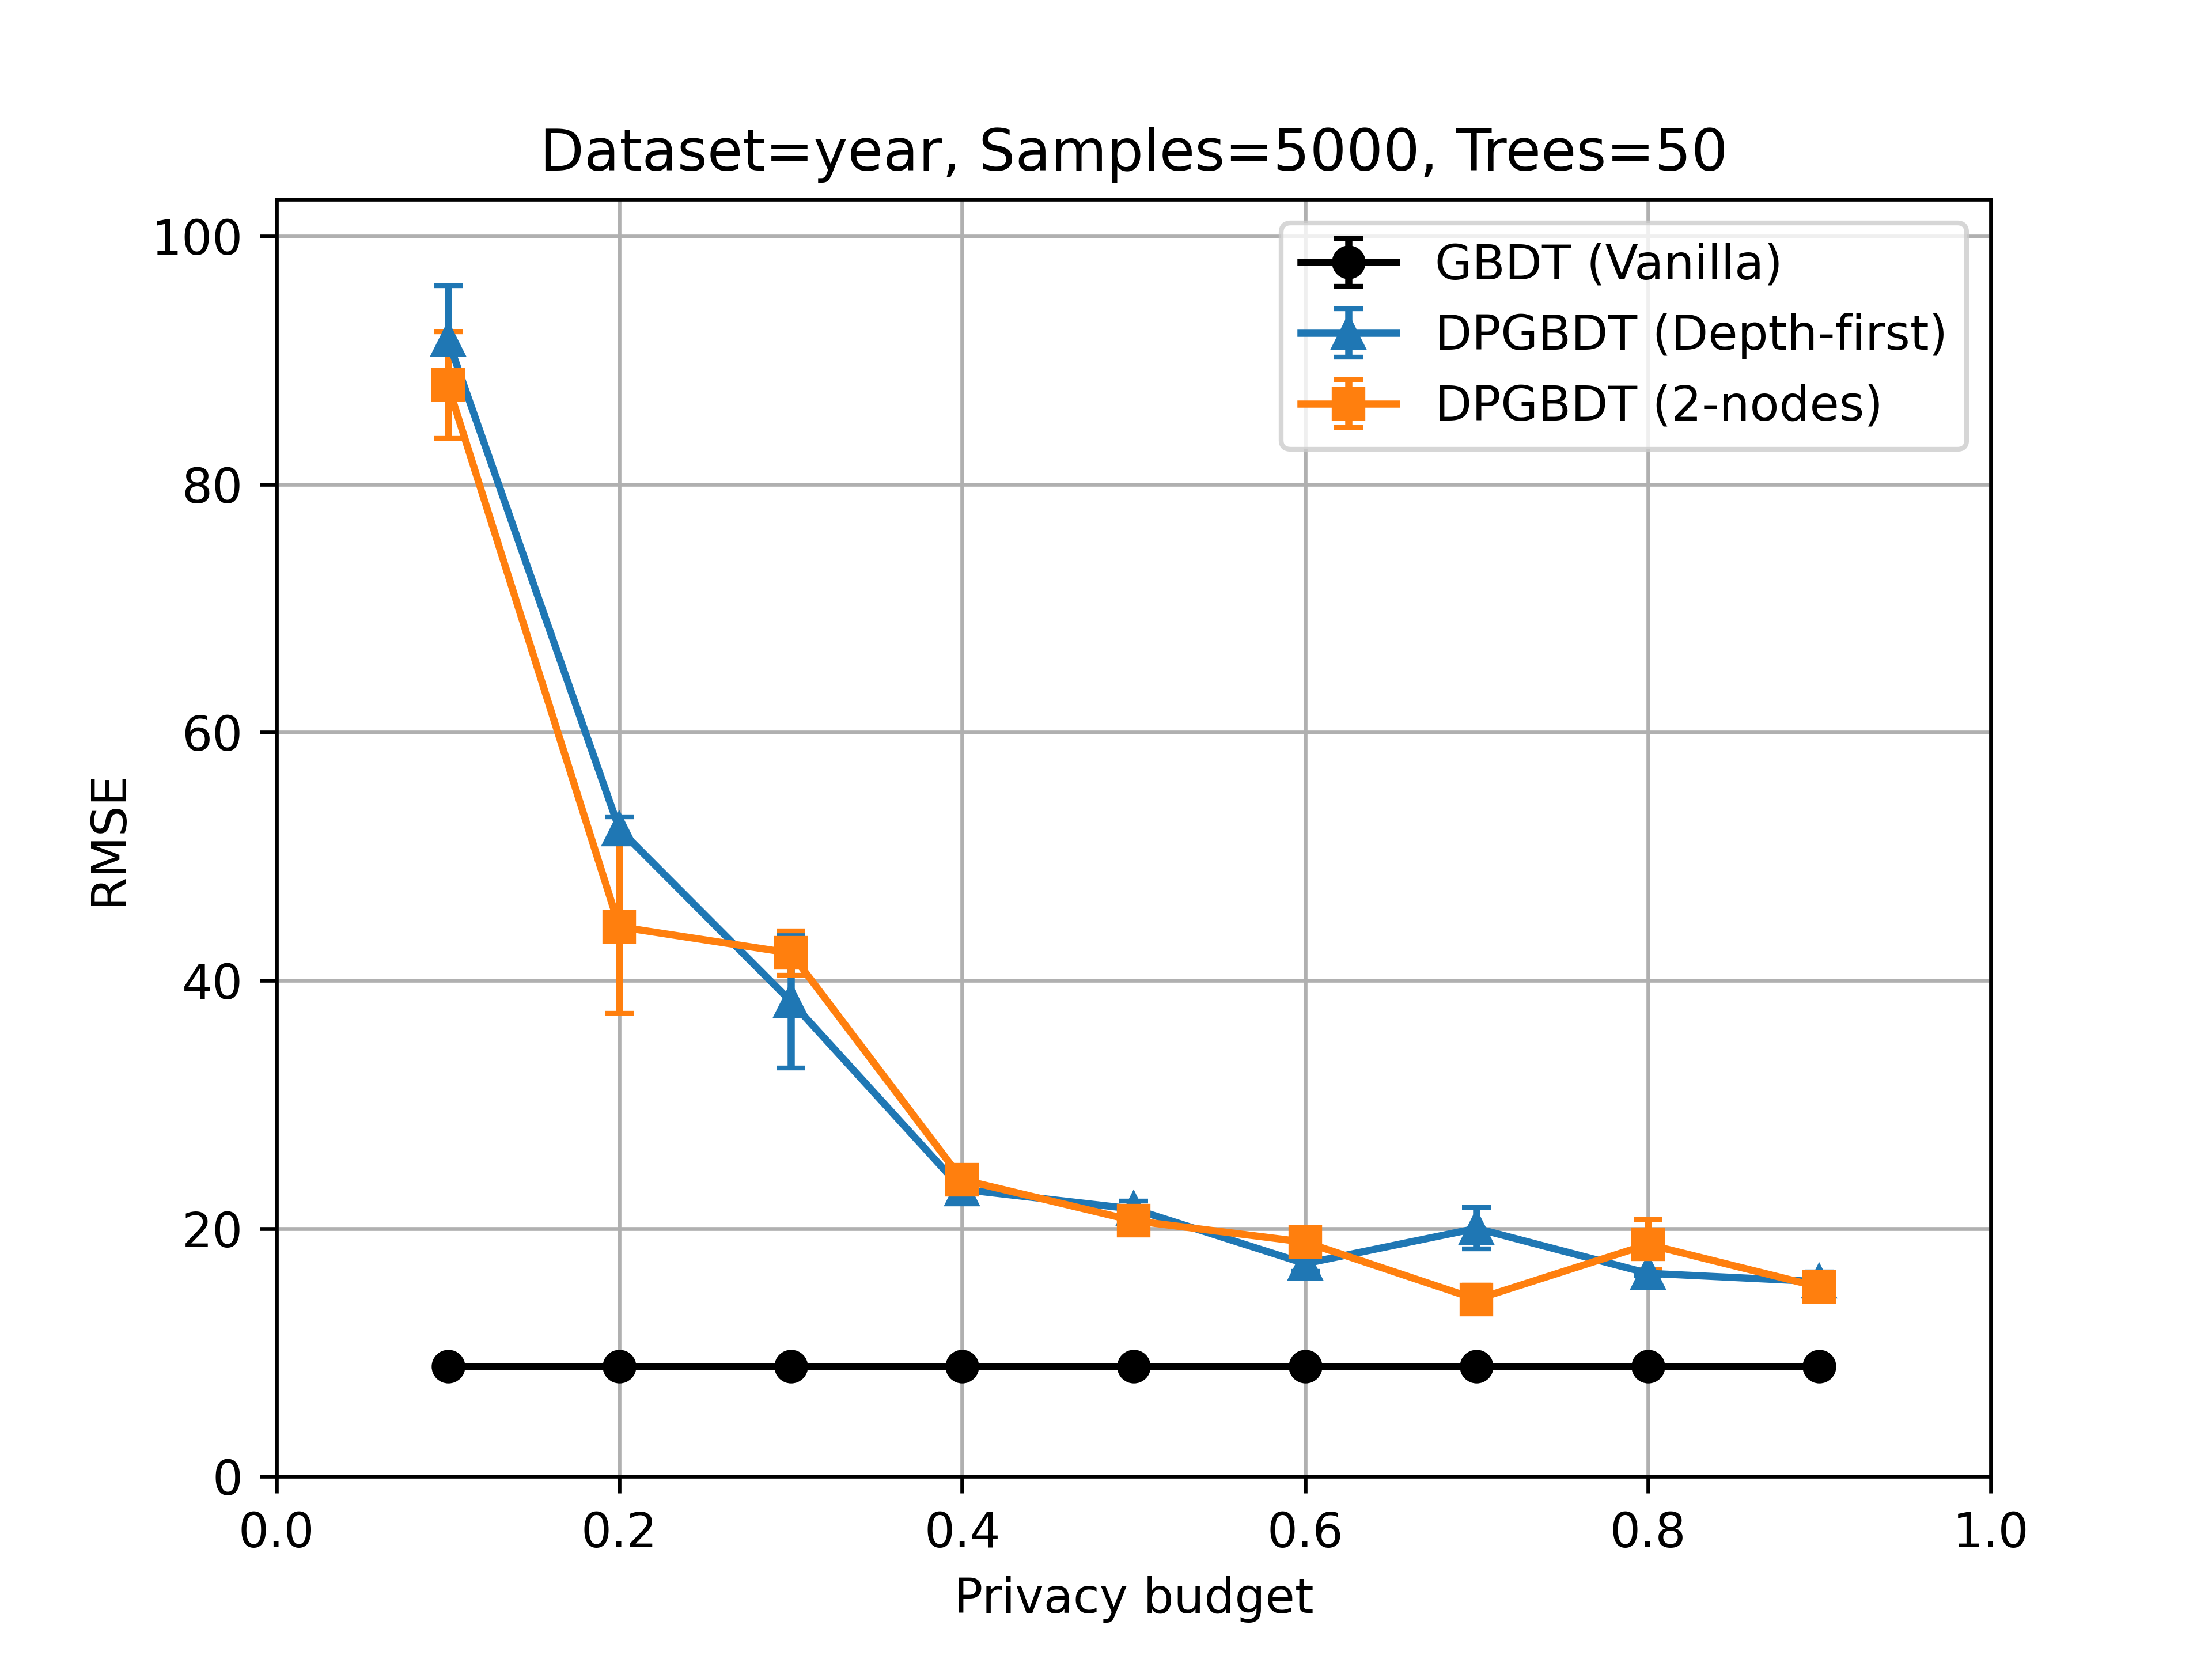
\includegraphics[width=.5\linewidth]{images/evaluation/year_5000.png}
  \caption{Regression tasks: Abalone and YearPredictionMSD}
  \end{subfigure}\par\medskip
  \begin{subfigure}{\linewidth}
  \center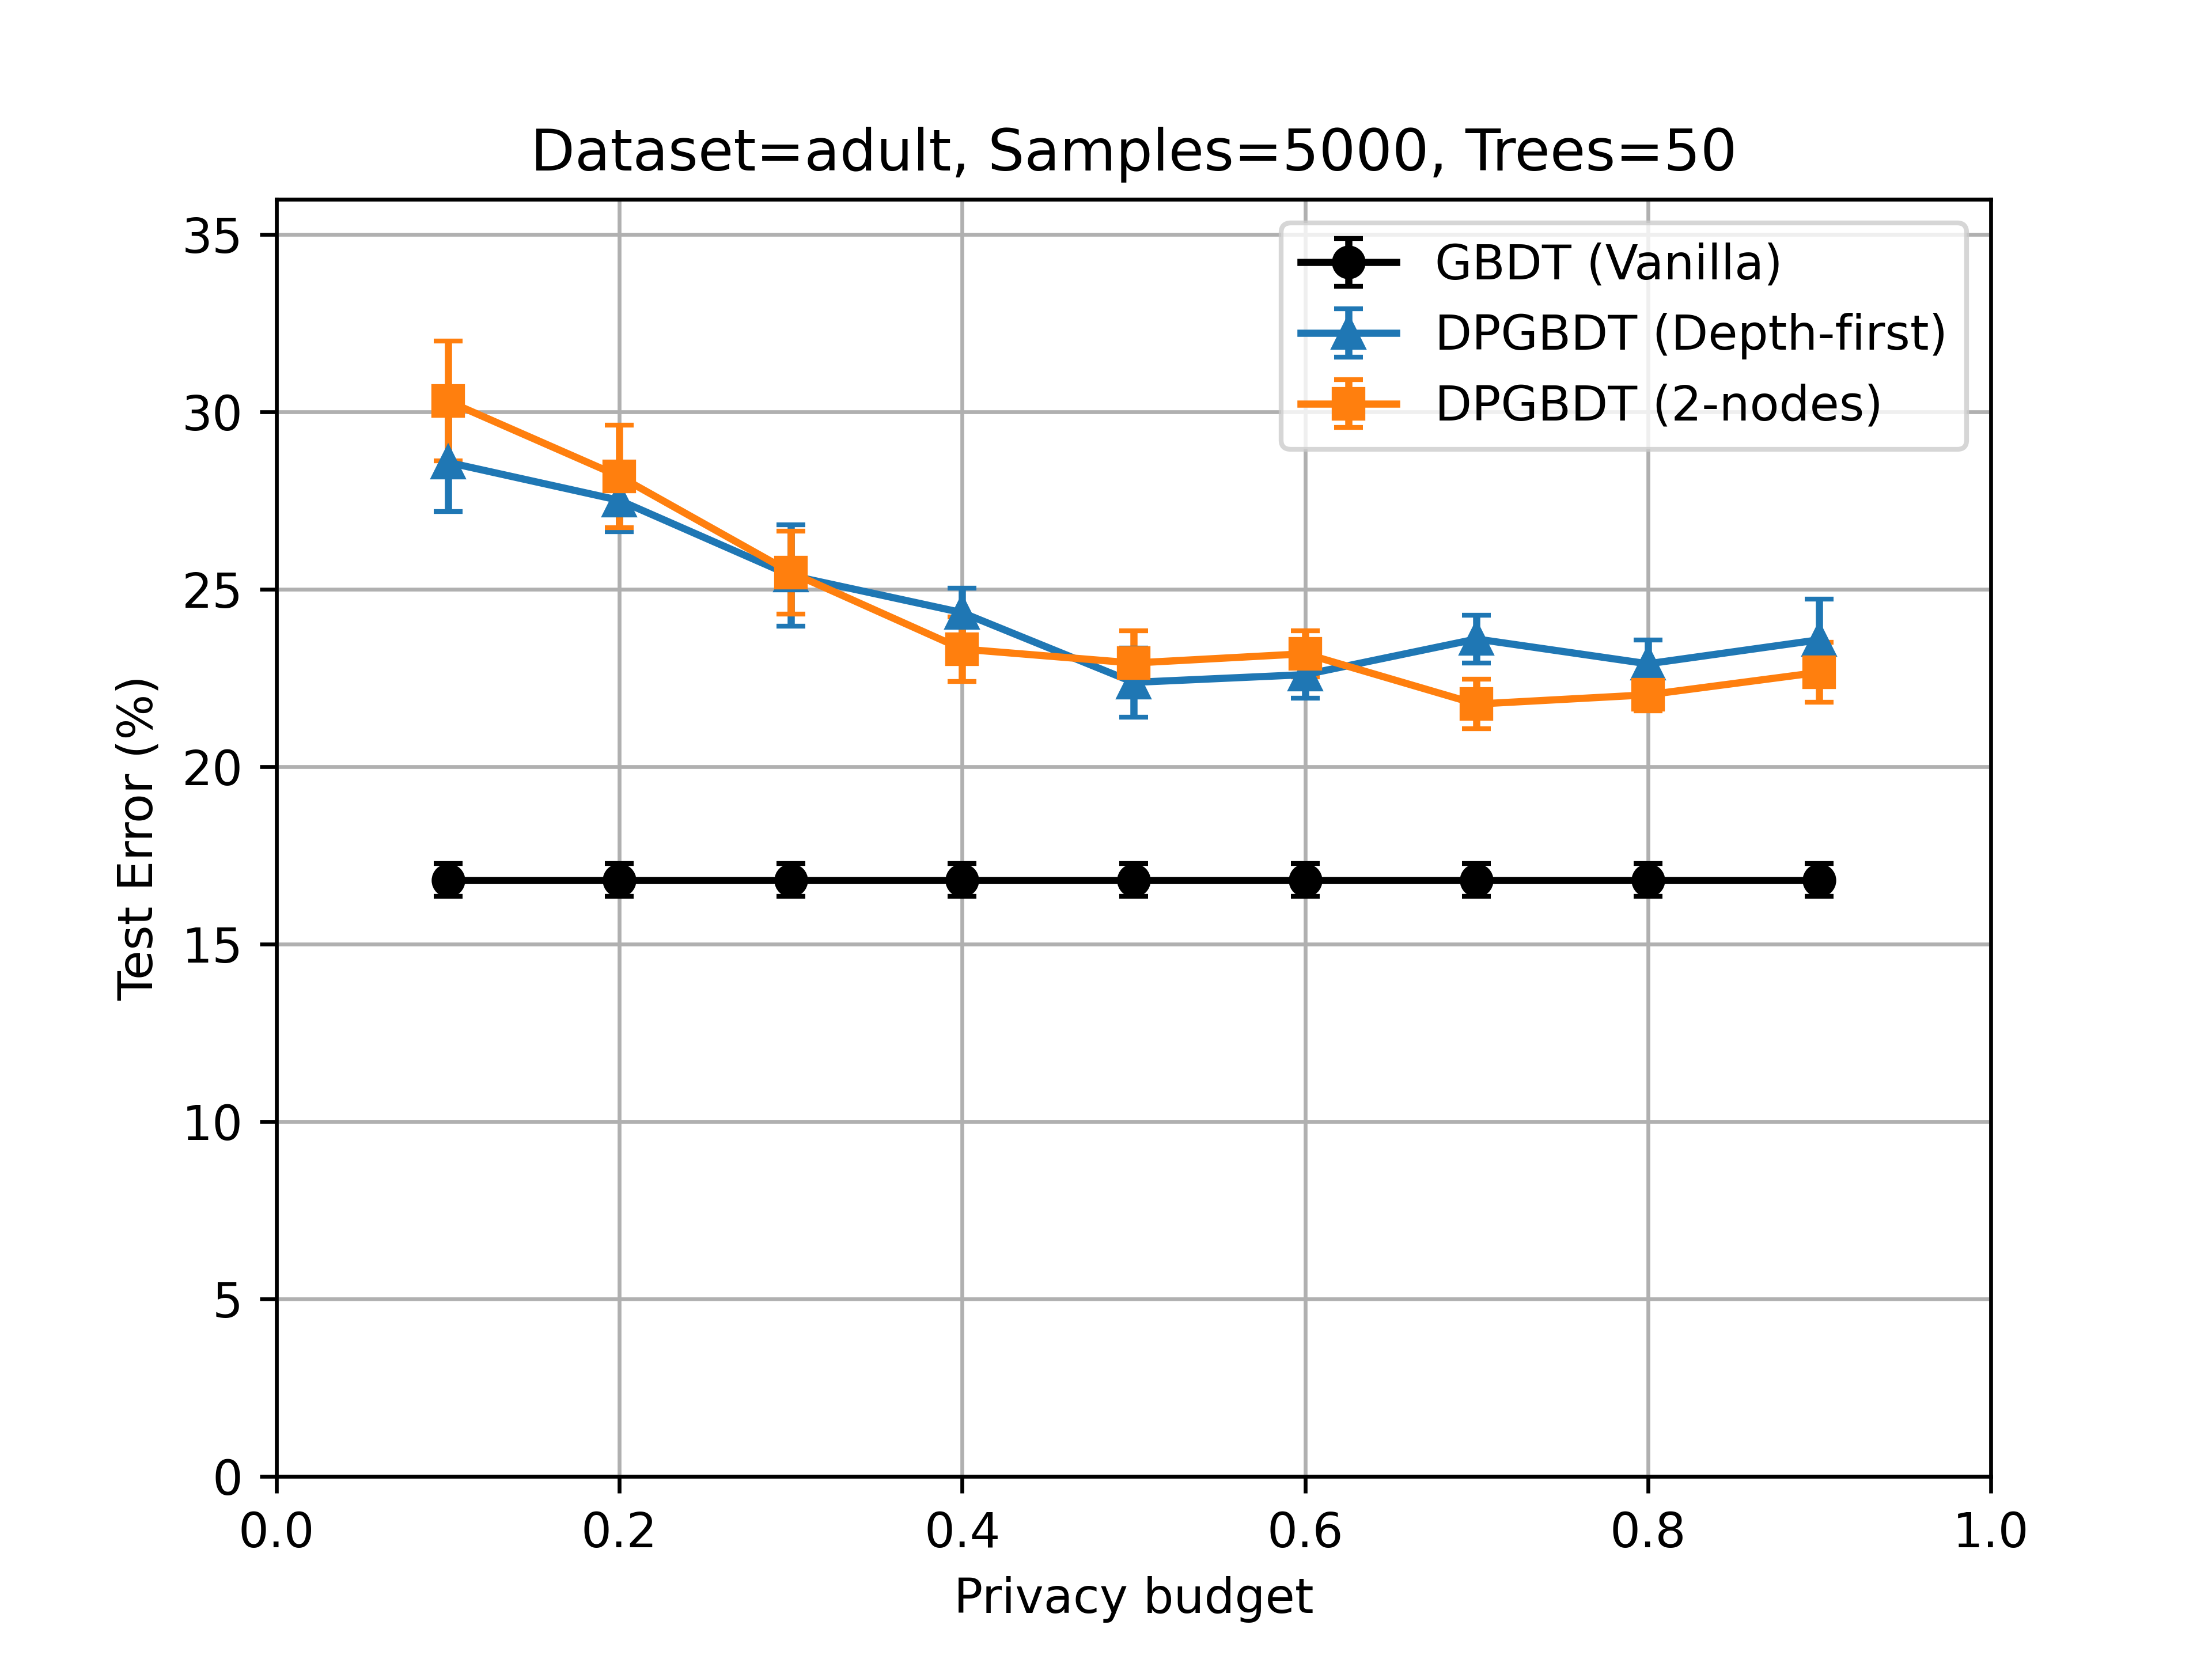
\includegraphics[width=.5\linewidth]{images/evaluation/adult_5000.png}
  \caption{Classification task: Adult}
  \end{subfigure}
  \caption{\label{fig:results_real}Prediction error for the vanilla model and various values of $\epsilon$ for the differentially private model.}
\end{figure}

\begin{figure}[h!]
	\center
	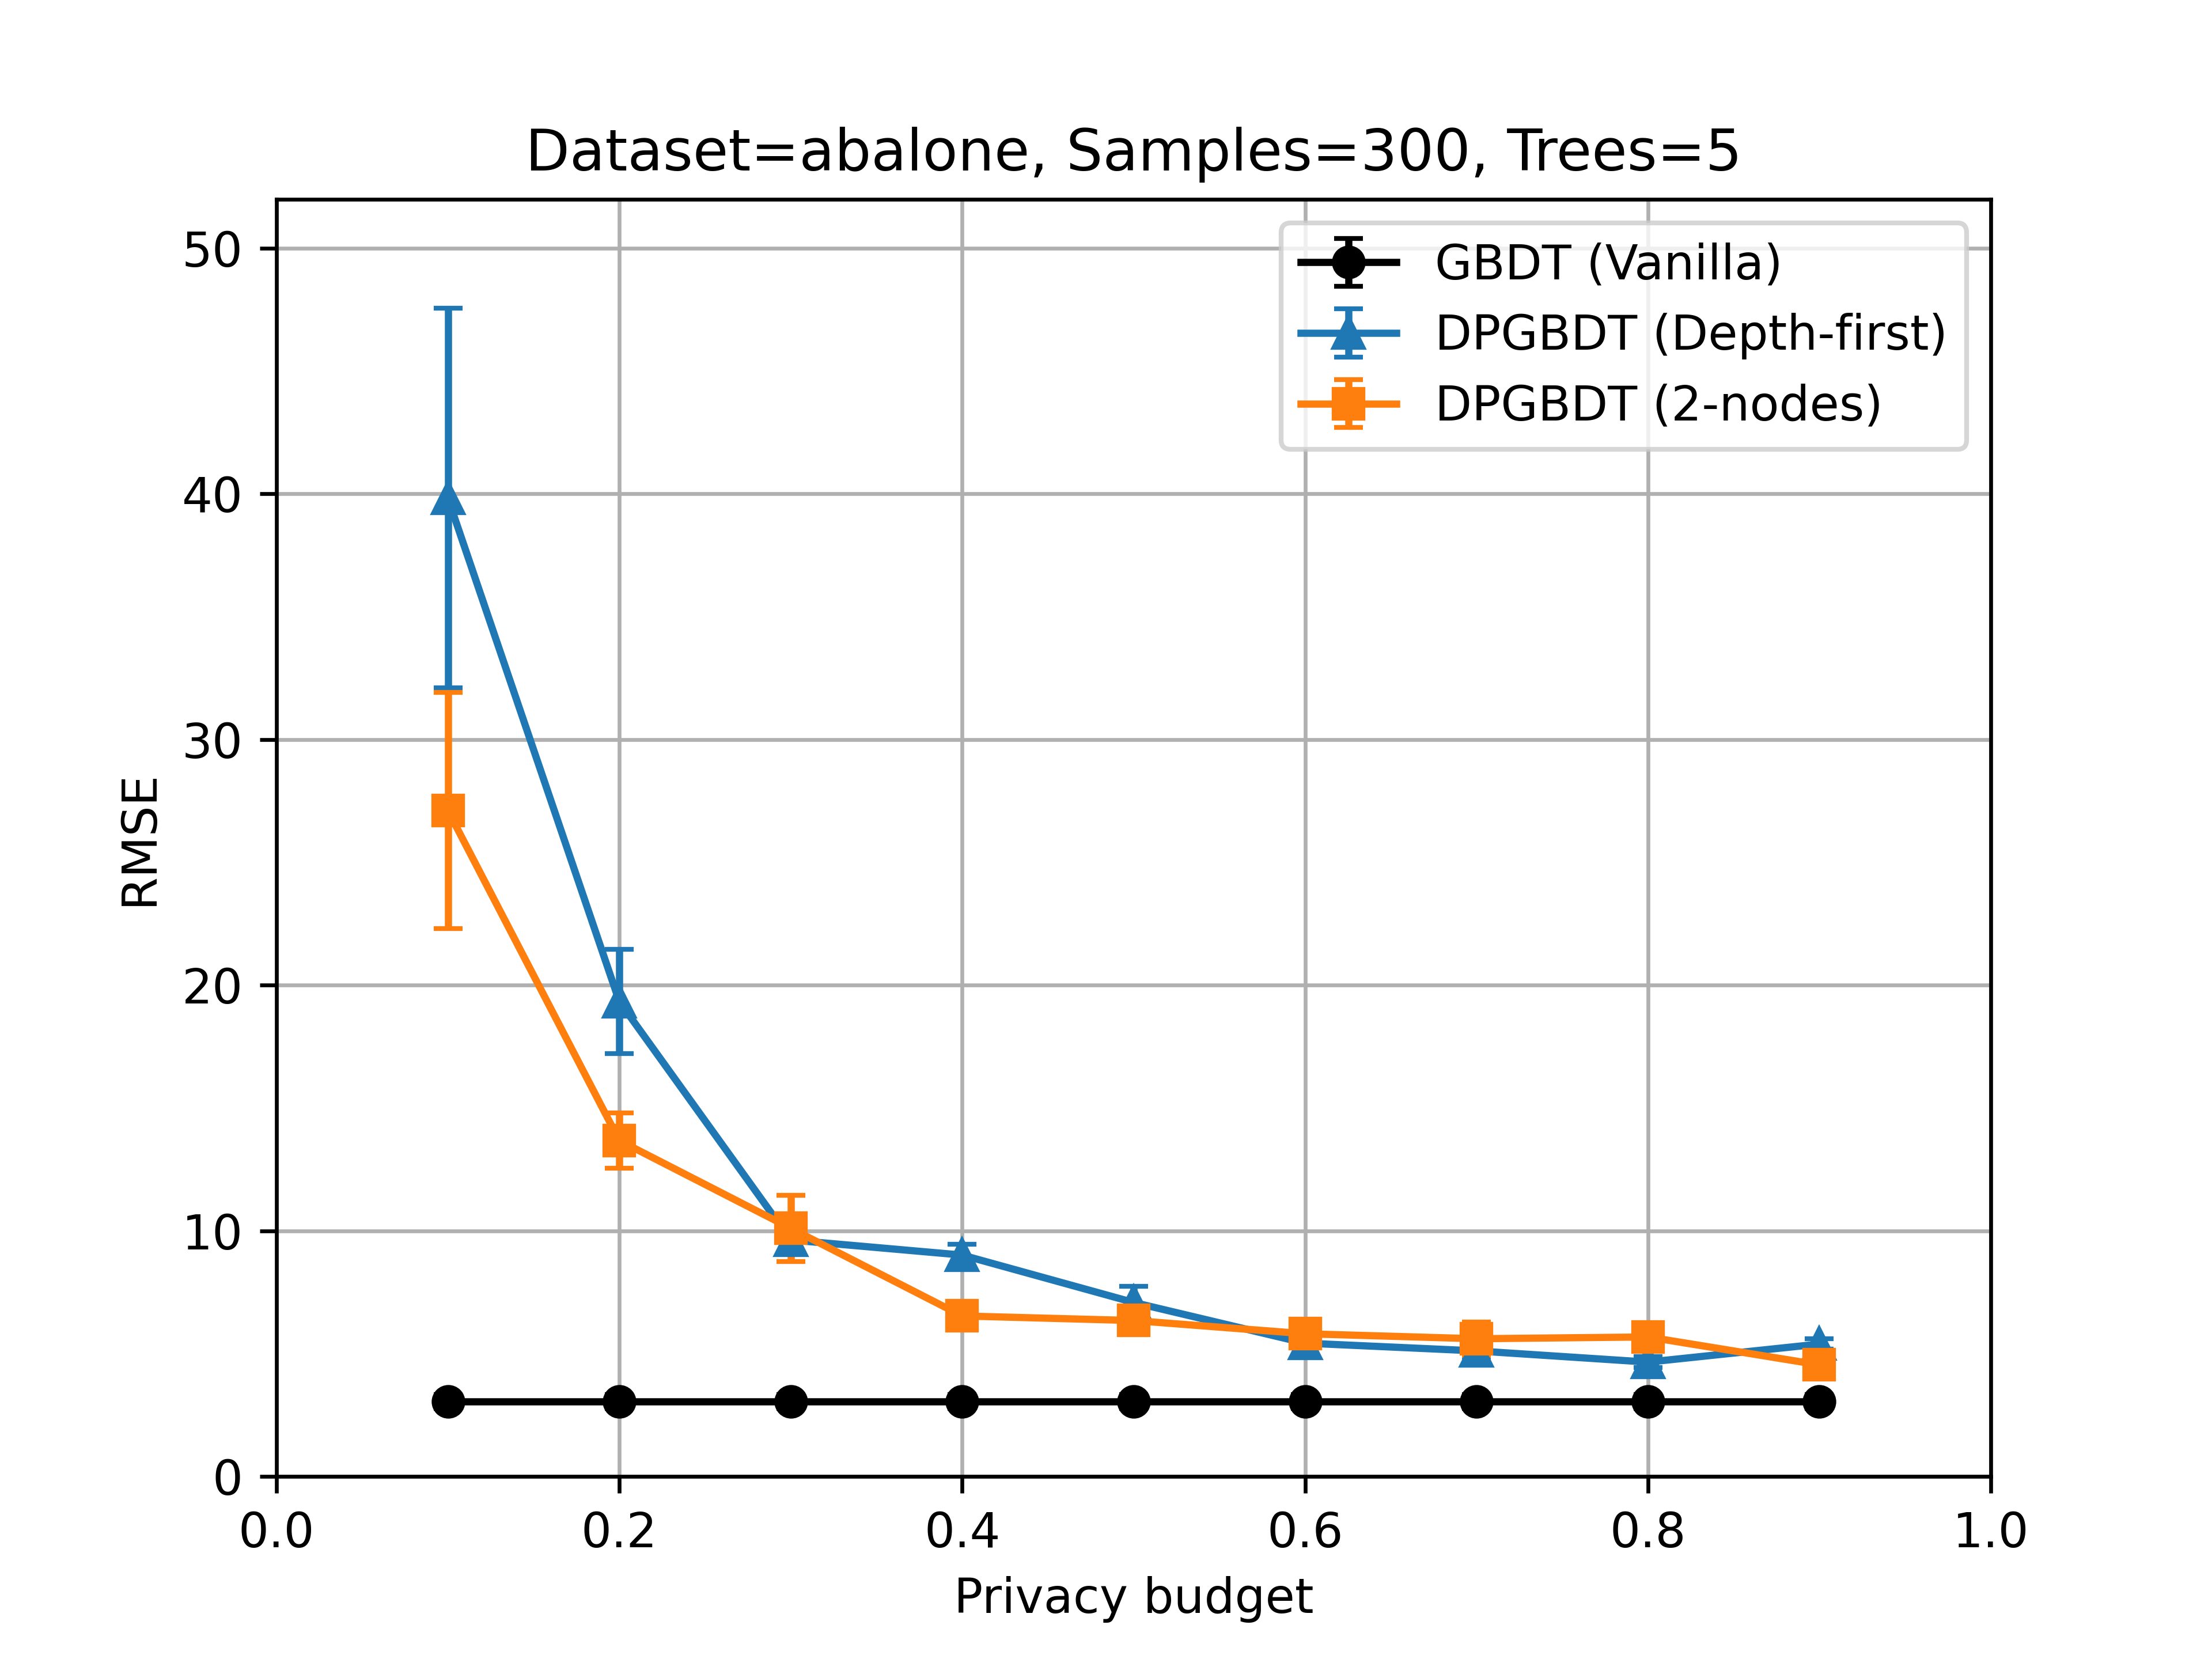
\includegraphics[width=.5\linewidth]{images/evaluation/abalone_300.png}
	\caption{\label{fig:abalone_300} Prediction error for the Abalone dataset, with 300 samples.}
\end{figure}

As shown in Figure ~\ref{fig:results_real}, our 2-nodes induction method performs slightly better than the regular depth-first induction method. This is especially visible in the Abalone dataset when $\epsilon$ is low and when we decrease the number of samples to $n = 300$ and the number of trees to $n_{trees} = 5$, where for $\epsilon=0.1$ our \textit{2-nodes} model performs $31.94\%$ better than the regular depth-first model. (reported in Figure ~\ref{fig:abalone_300}).

Table ~\ref{table:pred_results_real} summarises the results for the vanilla model versus the differentially private model (where the privacy budget is fixed to $\epsilon = 0.5$) on these real-life datasets.

\begin{center}\begin{table}[h!]
	\center
	\noindent\makebox[0pt]{}{
		\begin{tabular}{|c|c|c|c|}
 		\hline
 		 & (Non-DP) Vanilla & (DP) Depth-first & (DP) 2-nodes \\ [0.5ex] \hline\hline
 		Abalone (RMSE) & $2.15 \pm 0.04$ & $6.58 \pm 0.40$  & $\textbf{6.18} \pm \textbf{0.75}$ \\ \hline
 		YearPredictionMSD (RMSE) & $8.87 \pm 0.16$ & $21.57 \pm 0.64$ & $\textbf{20.62} \pm \textbf{0.13}$ \\ \hline
 		Adult (Test error) & $16.81 \pm 0.45$ & $\textbf{22.37} \pm \textbf{0.97}$ & $22.92 \pm 0.91$ \\ \hline
	\end{tabular}
	\caption{\label{table:pred_results_real} Prediction error for the real datasets.}}
\end{table}\end{center}

\newpage

For the synthetic datasets, we report the MAPE, defined as $MAPE = \frac{1}{n}\sum_{i}^n \abs{\frac{R_i - P_i}{R_i}}$ where $R_i$ is the real value and $P_i$ the predicted one. If the prediction task was to predict the price of an object, with its real price being $100\$$ and the predicted price being $110\$$, then the MAPE score would be $MAPE = \abs{\frac{100-110}{100}} = 0.1$ i.e. $10\%$ error, since we would be $10\$$ off. 

Results for the \textit{cost} target are reported in Figure ~\ref{fig:results_synthetic_cost}. For the \textit{loss} target, the reader can refer to Figure ~\ref{fig:results_synthetic_loss}. Table ~\ref{table:pred_results_synthetic_cost} summarises the results for the vanilla model versus the differentially private model (where the privacy budget is fixed to $\epsilon = 0.5$), for the \textit{cost} target. For the \textit{loss} target, the reader can refer to Table ~\ref{table:pred_results_synthetic_loss}.

\begin{center}\begin{table}[h!]
	\center
	\noindent\makebox[0pt]{}{
		\begin{tabular}{|c|c|c|c|}
 		\hline
 		 & (Non-DP) Vanilla & (DP) Depth-first & (DP) 2-nodes \\ [0.5ex] \hline\hline
 		Synthetic A (MAPE) & $2.90 \pm 0.80$ & $11.83 \pm 3.31$  & $\textbf{7.12} \pm \textbf{0.89}$ \\ \hline
 		Synthetic B (MAPE) & $2.69 \pm 0.79$ & $8.43 \pm 1.62$  & $\textbf{7.99} \pm \textbf{1.58}$ \\ \hline
 		Synthetic C (MAPE) & $2.13 \pm 0.36$ & $\textbf{6.88} \pm \textbf{0.71}$  & $8.52 \pm 1.74$ \\ \hline
 		Synthetic D (MAPE) & $2.05 \pm 0.16$ & $7.00 \pm 0.76$  & $\textbf{5.47} \pm \textbf{0.42}$ \\ \hline
	\end{tabular}
	\caption{\label{table:pred_results_synthetic_cost} Prediction error for the \textit{cost} target on the synthetic datasets.}}
\end{table}\end{center}

For the synthetic dataset A, 2-nodes is able to decrease the error by almost $40\%$. For datasets B and D, the error decreases by $5.22\%$ and $27.97\%$ respectively. On dataset C, 2-nodes performs worst with an error increase of $23.84\%$.

%\newpage

\begin{figure}[h!]
  \begin{subfigure}{\linewidth}
  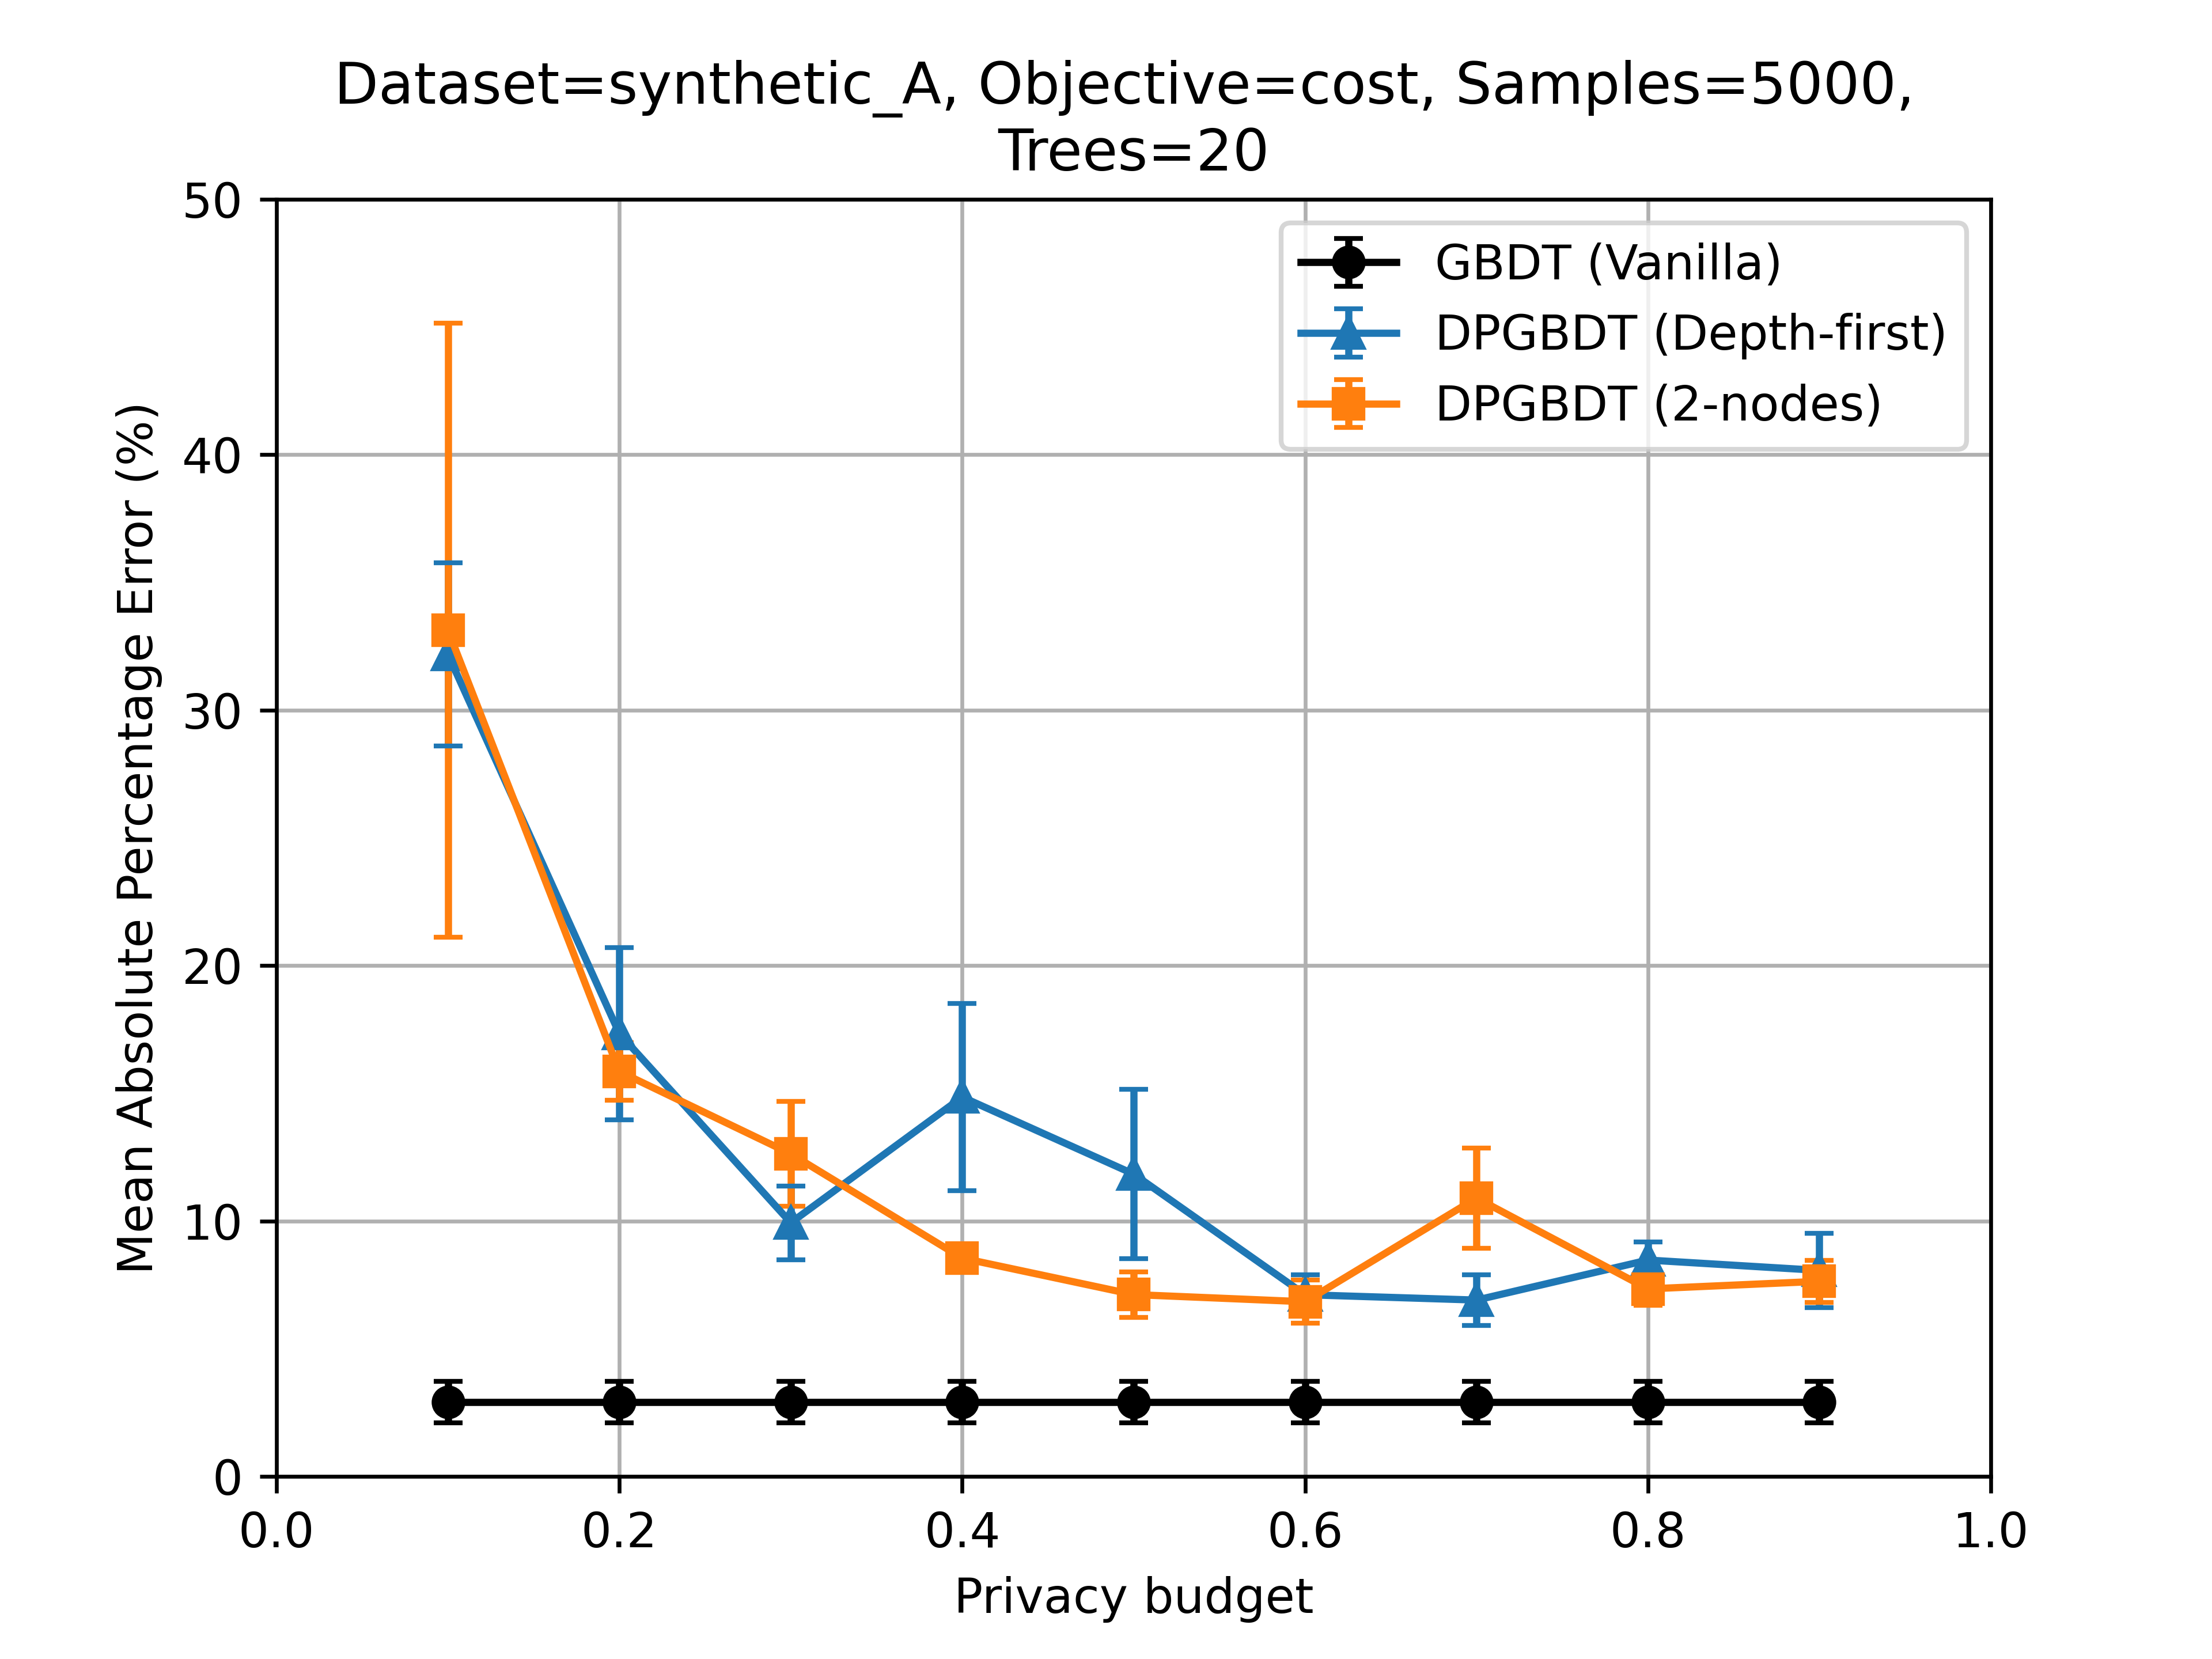
\includegraphics[width=.5\linewidth]{images/evaluation/synthetic_A_cost_5000.png}\hfill
  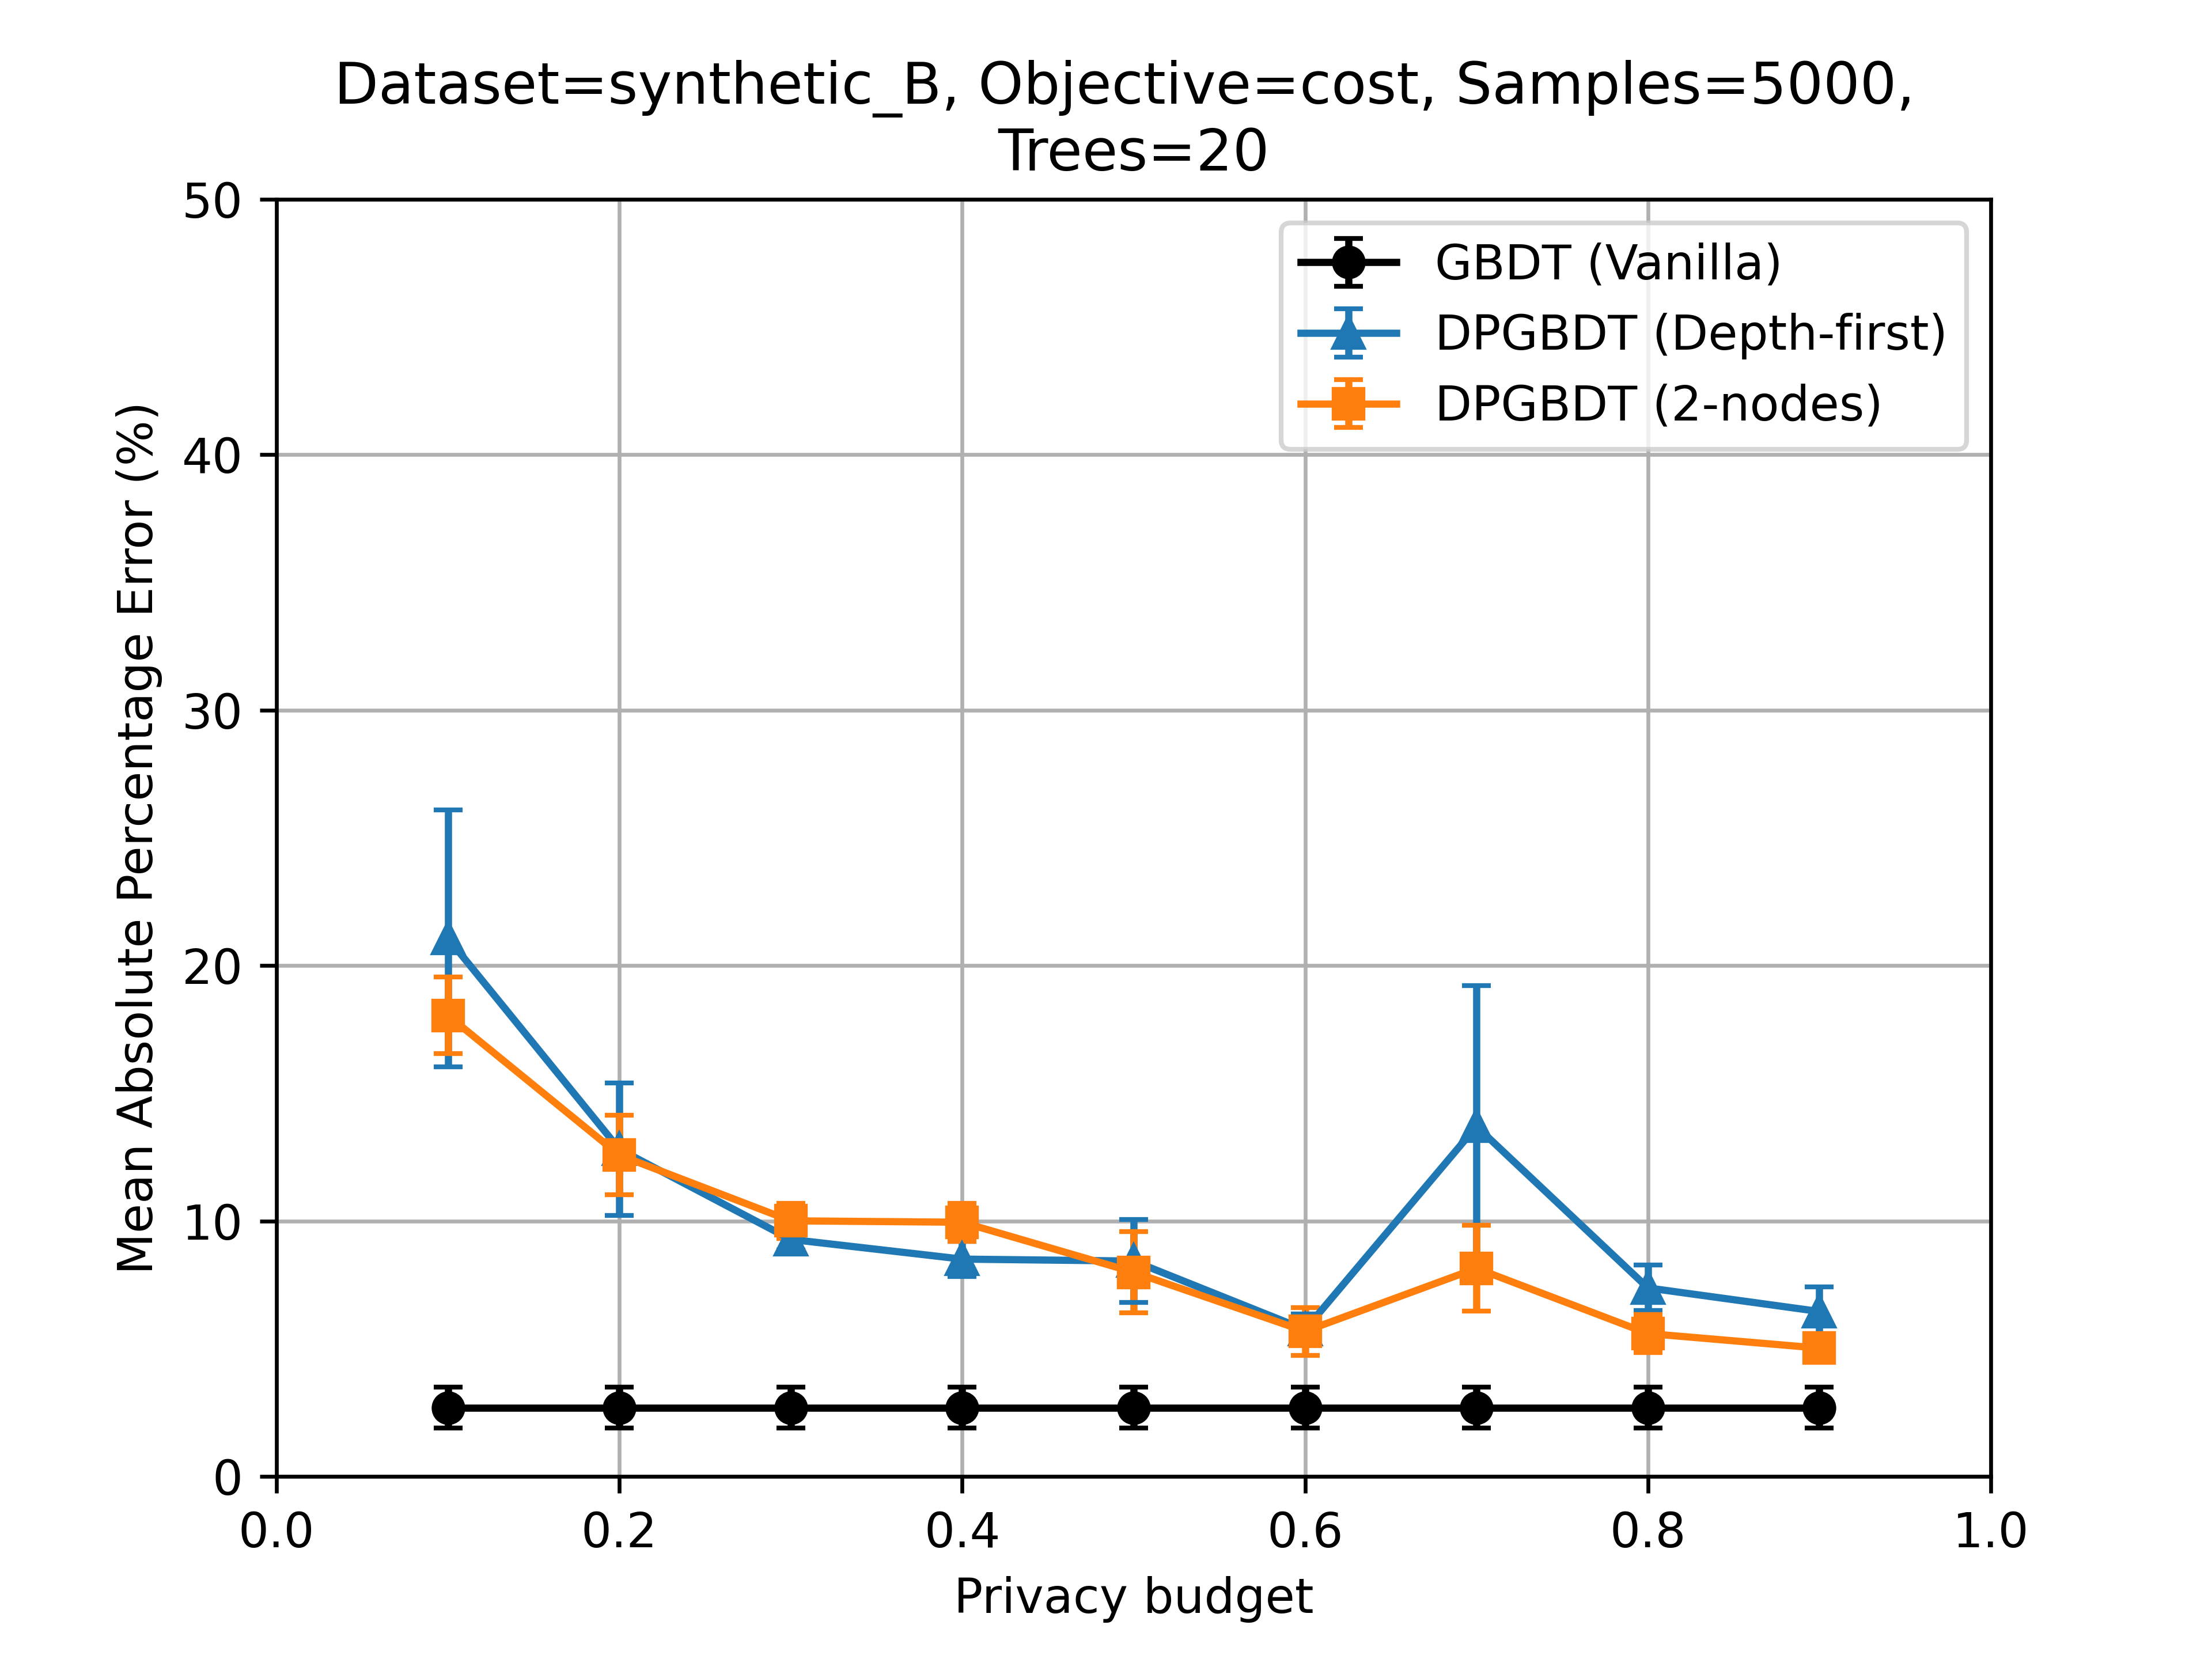
\includegraphics[width=.5\linewidth]{images/evaluation/synthetic_B_cost_5000.png}
  \caption{Synthetic datasets A and B}
  \end{subfigure}\par\medskip
  \begin{subfigure}{\linewidth}
  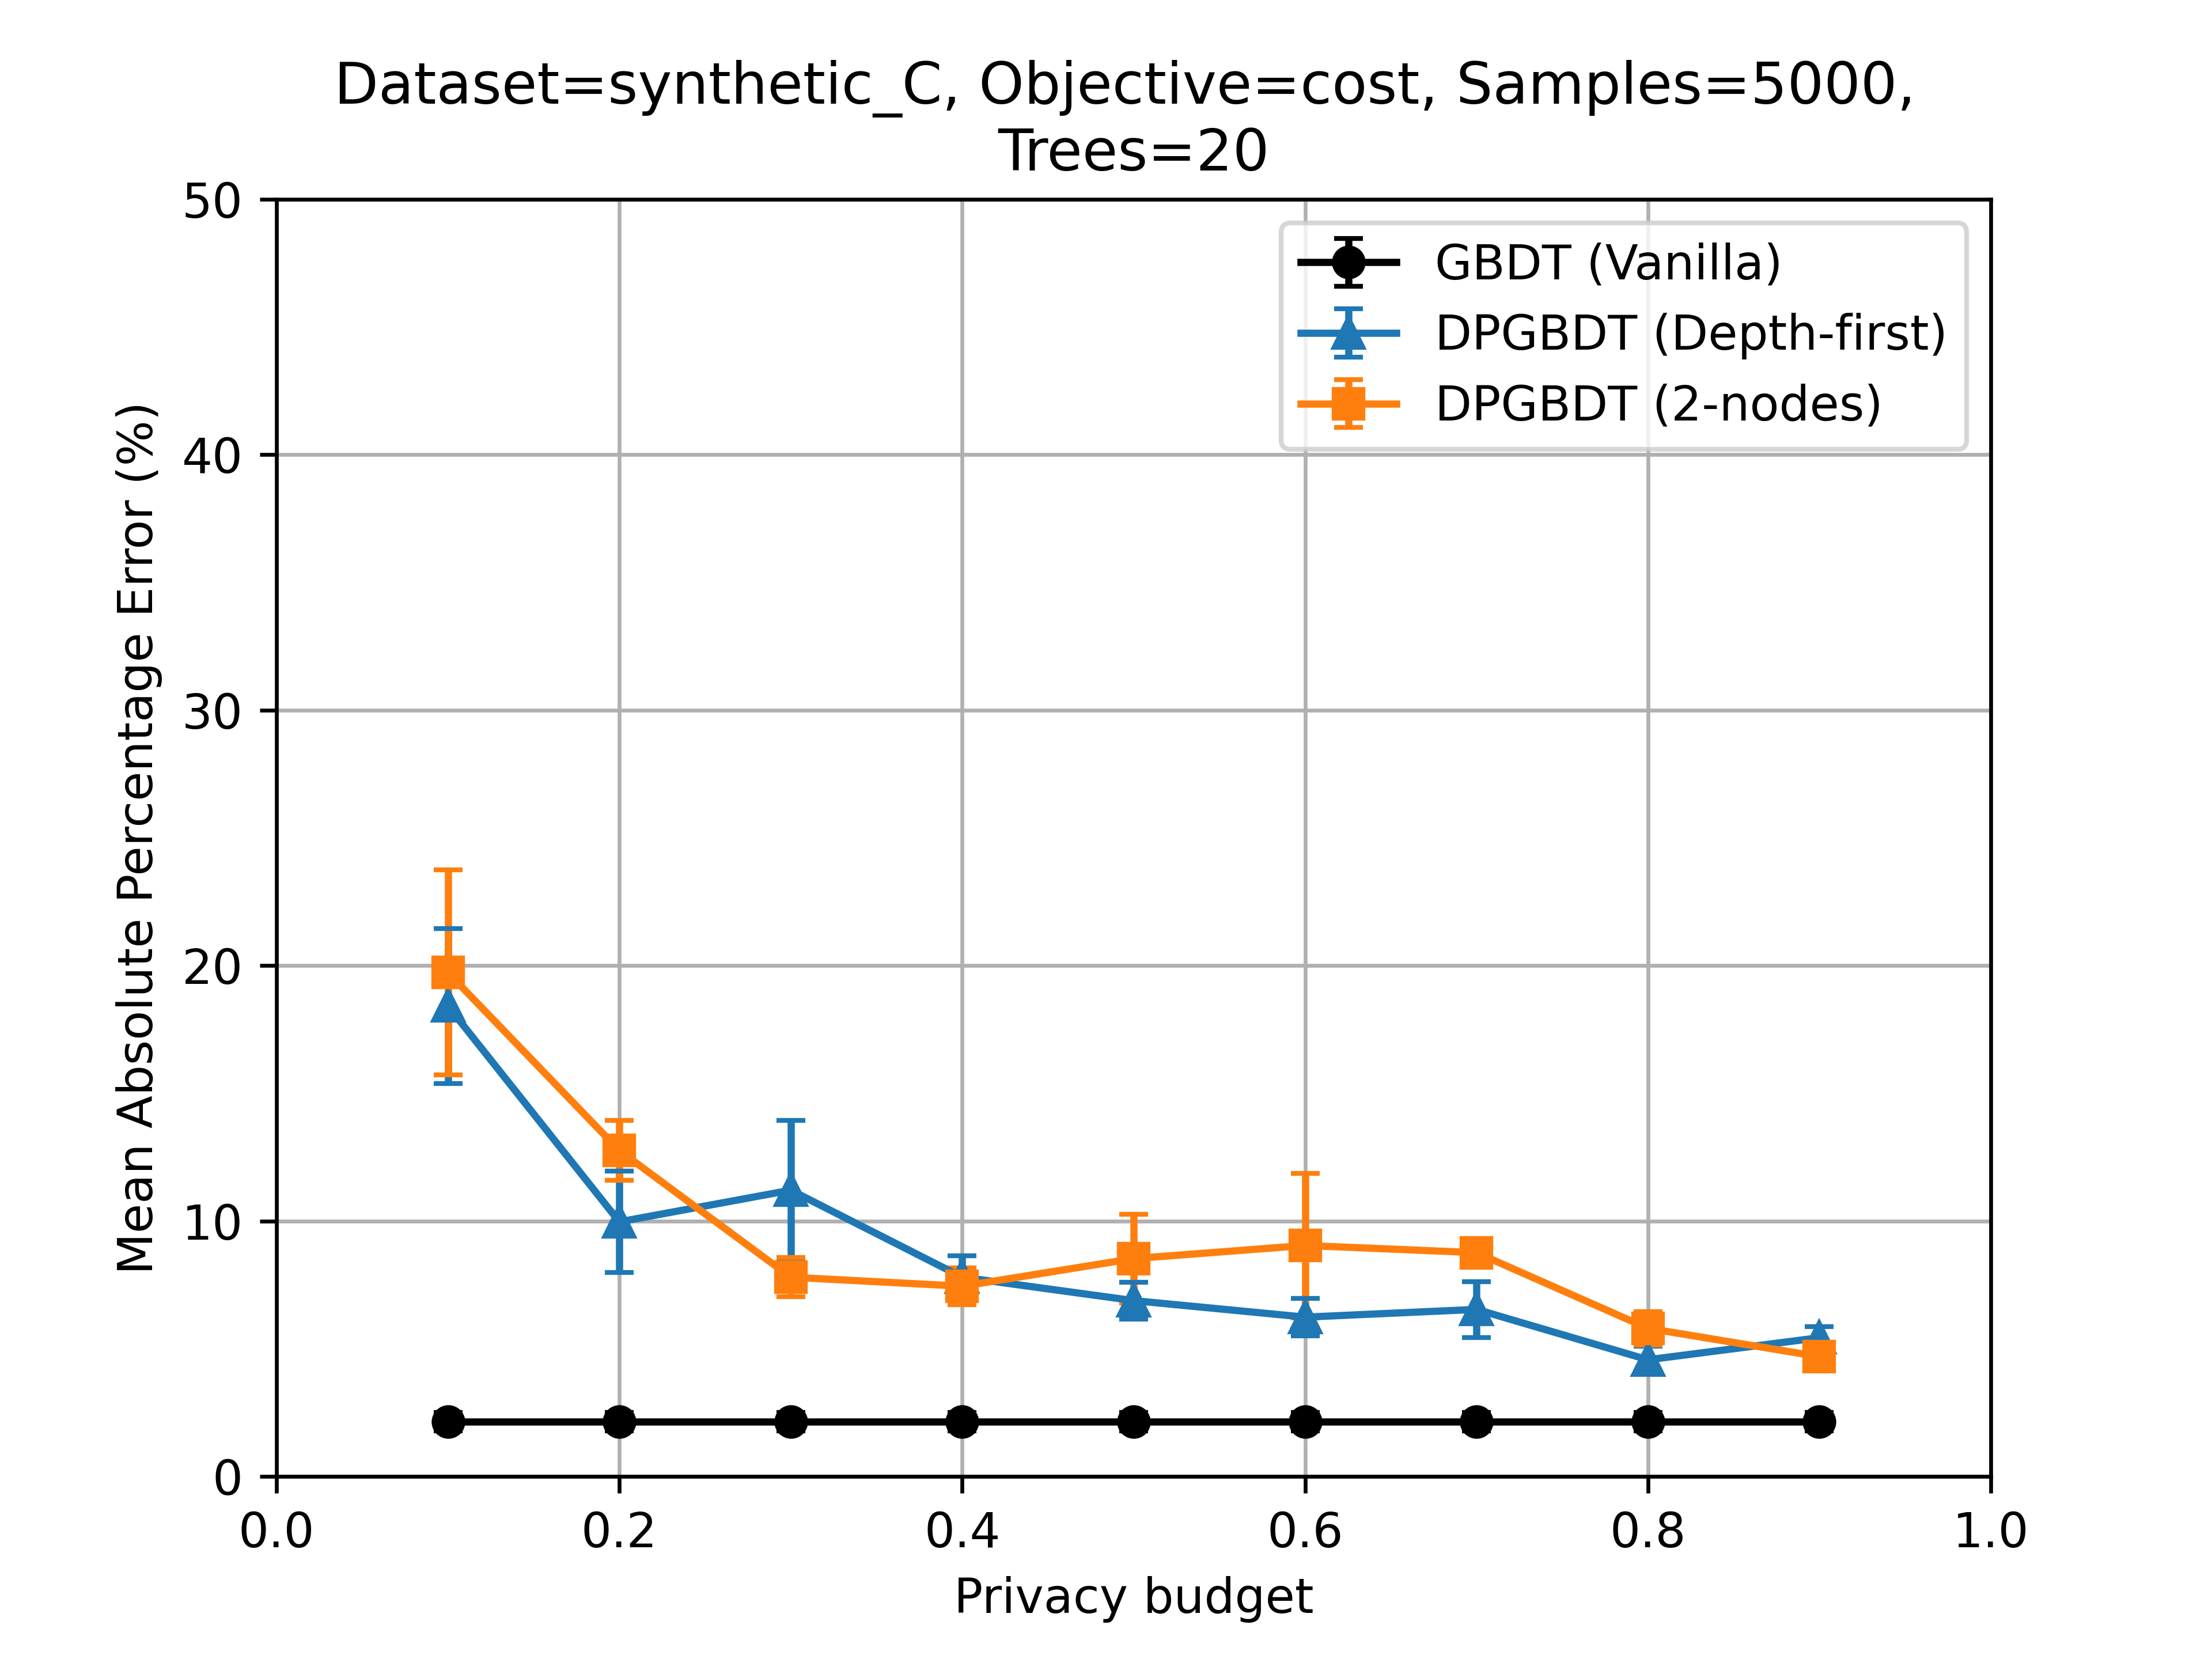
\includegraphics[width=.5\linewidth]{images/evaluation/synthetic_C_cost_5000.png}\hfill
  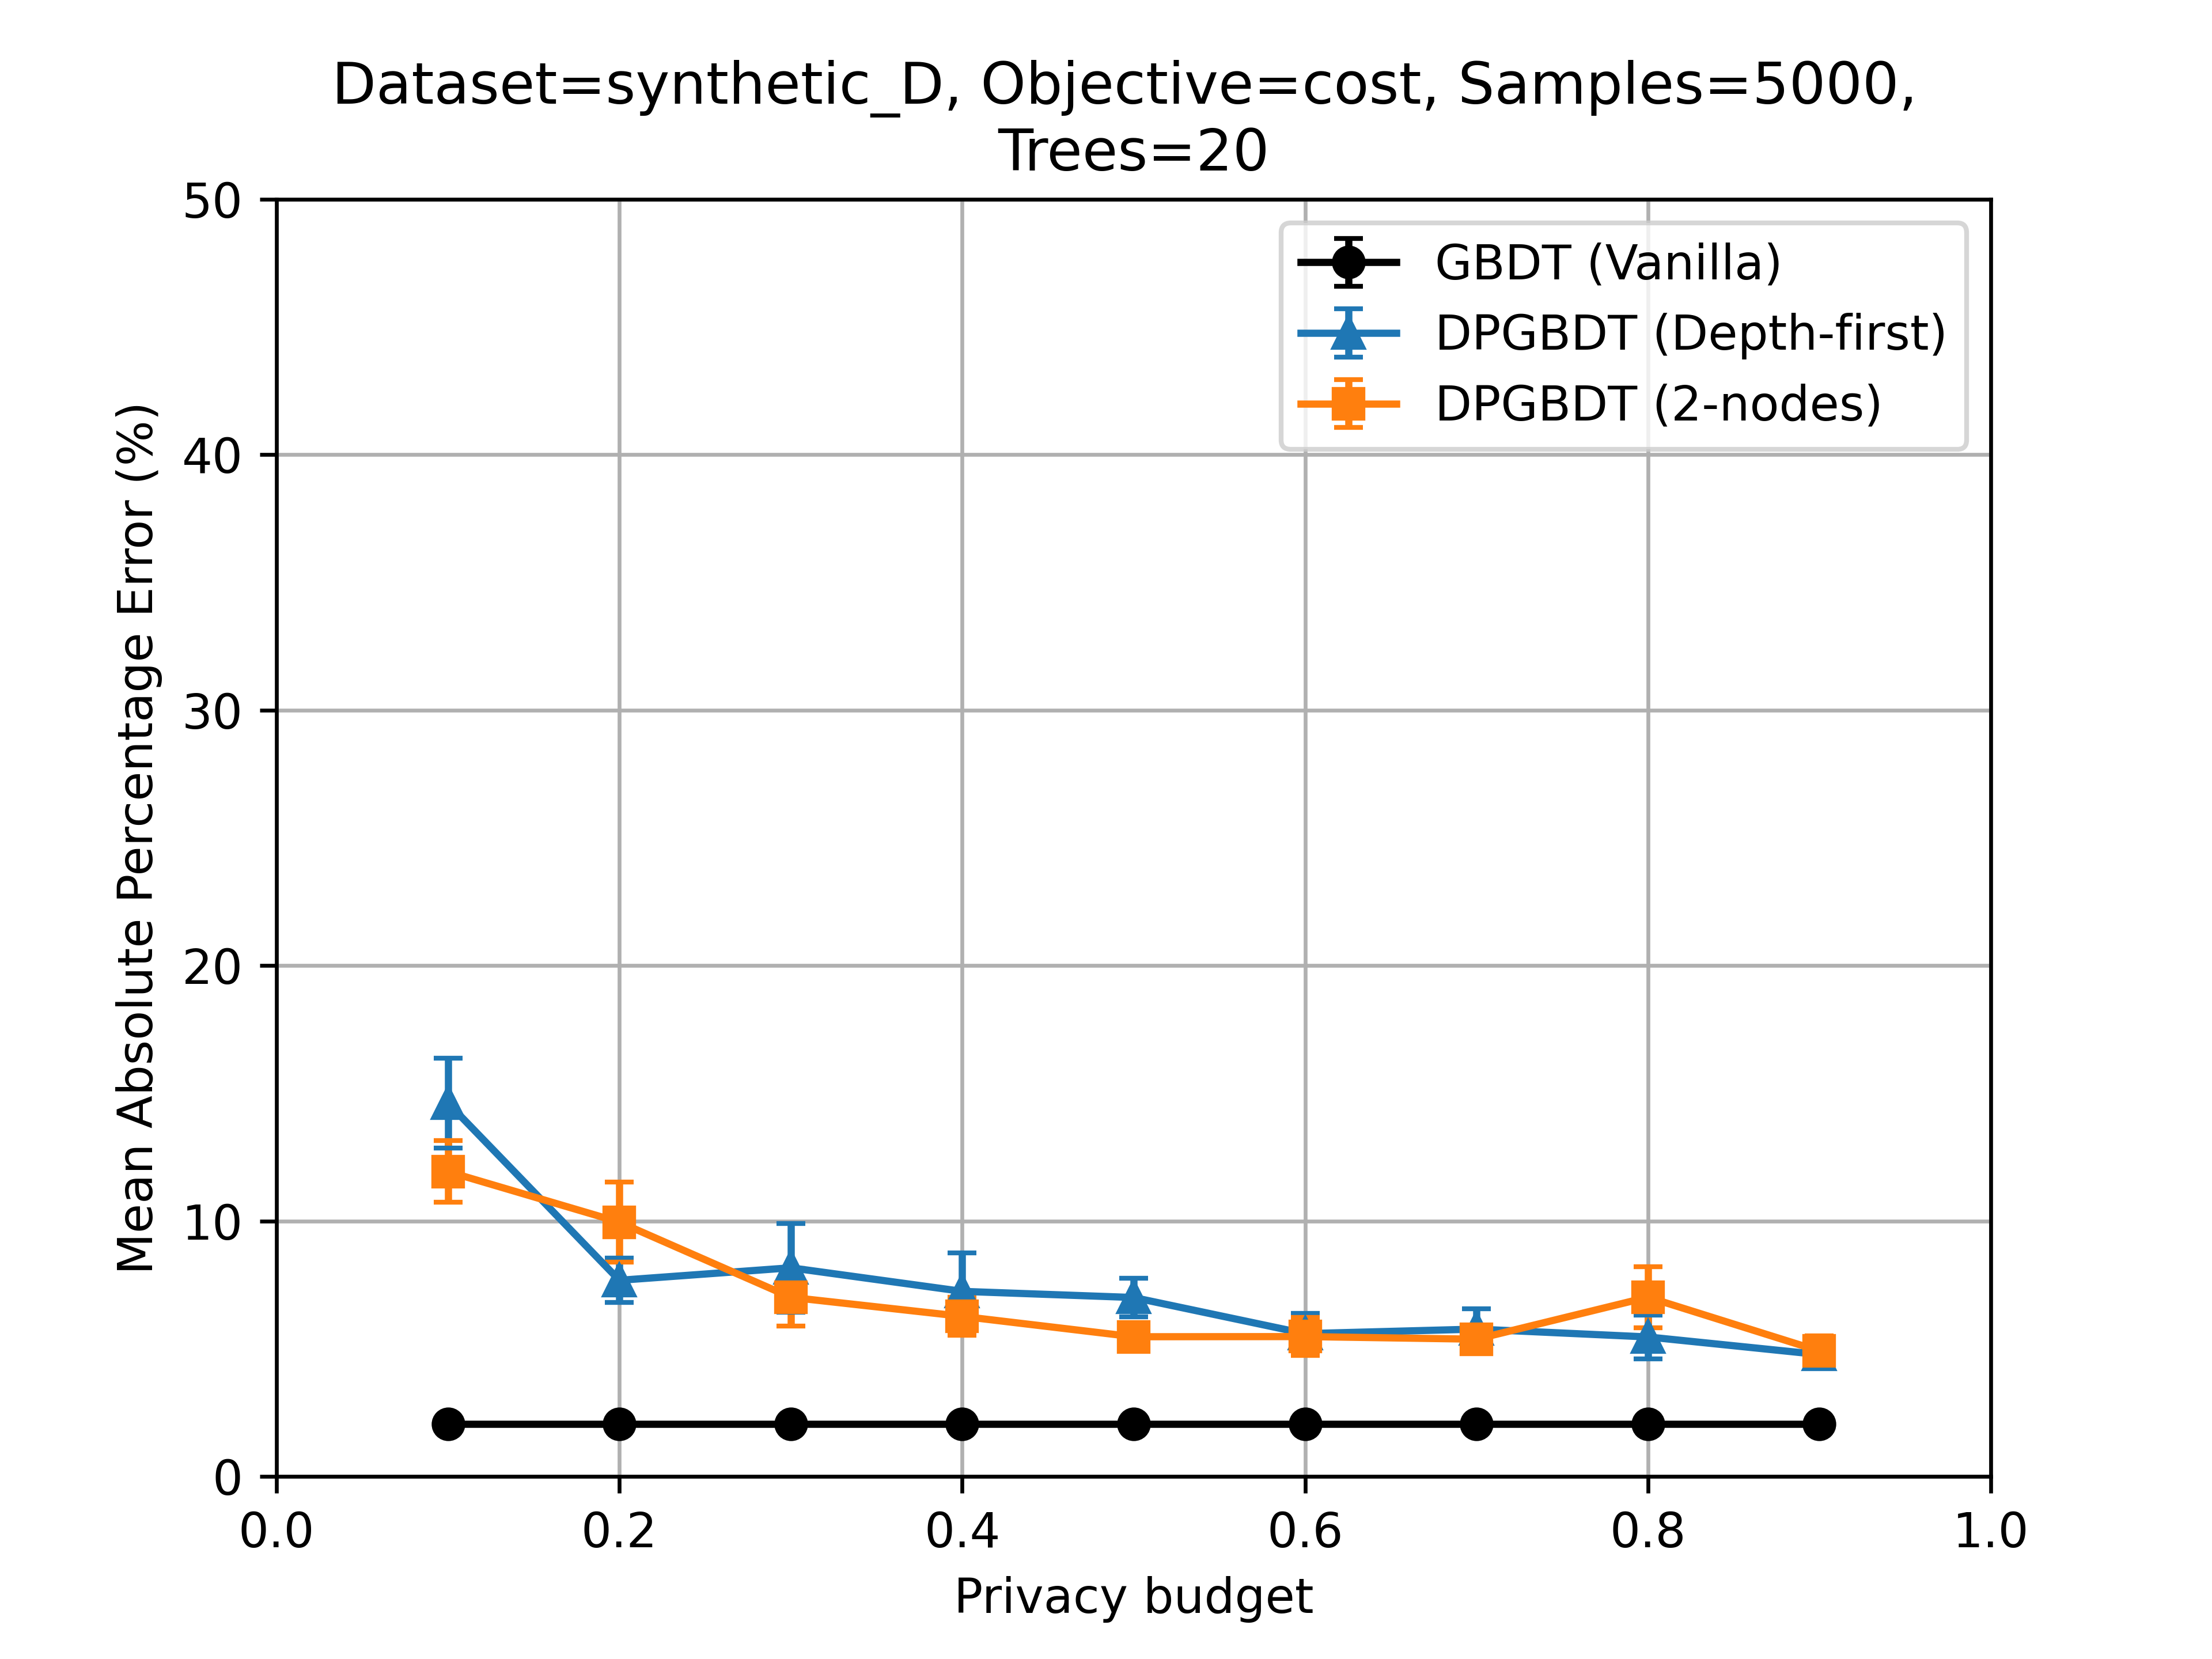
\includegraphics[width=.5\linewidth]{images/evaluation/synthetic_D_cost_5000.png}
  \caption{Synthetic datasets C and D}
  \end{subfigure}
  \caption{\label{fig:results_synthetic_cost}Mean Absolute Percentage Error for the \textit{cost} target on the synthetic datasets.}
\end{figure}
